\chapter{Financial Study}

The different departments have estimated the main costs of the project. It is high time to start performing a deep analysis on the economical solvency of the project. The analysis carried on will be of 10 years. 

Up to this point, it is important to determine how this product will be sold, so as to quantify the benefits of the project and be able to determine some figures such as the Pay Back Time or the Net Present value, and be able to make some conclusions. 

\section{Selling the product}

The aim of the project is to be able to sell to the customers the chance of both sending and receiving data from satellites. Therefore, it seems logic that the price of the product has to be somehow related to the amount of data passed on. Then, there will be a price for every Mbit, either sent or received. 

From the Communications Department, there is a limitation of 3 Ground Stations operating, and each one can carry up to 25 Mbits/second. Accepting that those Ground Stations will fully operating the whole year, and calculating the amount of seconds that there are in a normal year:
\begin{equation}
365 \cdot 24 \cdot 60 \cdot 60 = 31536000 s
\end{equation}
It can be easily calculated the amount of Mbits that Astrea Constellation is able to either send or receive:
\begin{equation}
31536000 \cdot 75 = 2365200000 Mbits
\end{equation}
This means that no more than 2365200000 Mbits can be sold. This is the maximum supply.

But how can the demand be estimated? There is a need to make assumptions. 

\subsection{Estimation of demand}

\subsubsection{Universities}

Firstly, it has been thought that the service offered has great academic interests. In fact, any student could build a satellite with a certain payload, send it to space and then receive data from the satellite at any time thanks to Astrea constellation. 
\newline
\newline
In order to study the possible demand of Mbits, an estimation of the possible universities that would want to use the services has been done. Fortunately, the list of universities that offer studies in the aerospace field goes back a total of 400 schools approximately. Nevertheless, it is highly improbable that all those colleges become clients because not all universities have the same sources or interests. Therefore, the following list presents the number of existing colleges having an aerospace degree in each continent.

	\begin{table}[!h]
	\begin{center}
	\begin{tabular}{|c|c|}
	\bf{Continent} & \bf{Number of Universities}\\
	\hline 
	Europe & 124\\
	\hline 
	Asia & 138\\
	\hline 
	North America &  97\\
	\hline
	 South America & 18\\
	\hline 
	Australia & 8\\
	\hline 
	Africa & 12\\
	\end{tabular}
	\end{center}
	\caption{Table. List of Universities with Aerospace Degrees}
	\end{table} 	

By analyzing this information, it can be determined that the continents with countries with higher PIB have more colleges interested in the space field. It is noticed that Asia is the continent with more colleges because, even if it is mostly poor, it is so big that it has rich countries such as Japan, Korea or China and the United Arab Emirates. Moreover, Europe and North America are not so extensive but have a higher aerospace culture and interest. 
\newline
\newline
On the basis the service is affordable for many prestigious colleges and it permits to provide their students with the chance to improve their knowledge by doing their own experiments, it has been estimated that about 150 universities will end up contracting Astrea's service in the next years. If we assume that each university would be interested in sending or receiving a total of 630720 Mbits anually, therefore the number of Mbits for universities, anually, will be of 94608000 Mbits.

\subsubsection{Particular customers}
Another extremely important sector of clients are the private ones. It is harder to make an assumption on the number of Mbits consumed by this sector. Nevertheless, some figures are needed in order to perform a good feasibility study. 

According to the Union of Concerned Scientists of the United States of America, right now there are about 1500 satellites orbiting around the Earth. But every day space technology is more affordable and feasible, which leads to think that in the next years a good figure of satellites would be of roughly 2000. Nonetheless, around 40\% of those missions would benefit of a faster communication with their satellites. As Astrea provides a very competitive price, it seems reasonable to think that a good percentage of those satellites would be interested. In order to be conservative, a 50\% of those would be potencial clients. This means that 400 full operating satellites would use Astrea, and assuming also than the average amount of data that those satellites would either send or receive anually is of 946080 Mbits, the number of Mbits for particular clients, anually, will be of 378432000 Mbits.

It can be checked that the sum of the amounts of Mbits for universities and for particular clients is lower than the maximum amount of Mbits due to the 3 Ground Stations (as has been stated before), this is, 2365200000 Mbits. In particular, it turns out to be a fifth of this quantity. 

\subsubsection{Demand}
Taking into account both the universities and the particular clients, and making a conservative assumption, the estimation of the demand, in Mbits, is of a fifth of the maximum capacity of Astrea, this is, 473040000 Mbits anually. Also, in order to simulate the unceirtainty of the company during the first years (as years pass, the company gets reputation and therefore its amount of clients also enlarges, a percentage is applied during the first years. This means that first year only a 75\% of the potential customers exposed before will be achieved, the second year a 80\%, and so on, until the sixth year, in which a 100\% is achieved. 

\subsection{Pricing the service}
The determination of the price is made upon the feasibility study, in order to get a reasonable Pay Back Time and benefit. Nevertheless, it is a fact that the fare of Astrea service must fulfill a condition: it has to be competitive. 

Comparing with some others constellations that offer a similar service, in order to provide a competitive fare, it seems reasonable a price per Mbit of no more than 0.5 \euro per Mbit, as an upper tape.  


\section{Economic Feasibility Report}

In order to perform the analysis on the economical solvency of the project, following there is a table which contains the main costs of the project, as well as the numerical operations that allow to calculate some important financial parameters, such as the Net Present Value (NPV), the Internal Rate of Retorn (IRR), the Simple Pay Back Time (PBT), the Updated Pay Back Time (UPBT) and the Break Even Point (BEP). From this data, some conclusions will be drawn.

Firstly, though, there is need to take into account some costs that are not included in the other departments, and which are key to analyzing the costs and benefits. 
\subsection{Previous costs}
\subsubsection{Engineering hours}
The engineering hours, which were specified in the Project Charter, are again synthesized in the following table:

\begin{longtable}{ccc}
\toprule
\rowcolor[gray]{0.65}
    \textbf{Engineering hours budget} & \textbf{Hours} & \textbf{Labor cost (\euro)} \\
    \midrule
    \endhead
\hline
\rowcolor[gray]{0.85}
	MANAGEMENT &  &  \\ \hline
	Meetings documentation &  &  \\ \hline
	Meetings & 340 & 6800 \\ \hline
	Meetings preparation &  &  \\ \hline
	Agendas & 10 & 200 \\ \hline
	Minutes & 10 & 200 \\ \hline
	Task Tracking and scheduling &  &  \\ \hline
	Project Charter & 170 & 3400 \\ \hline
	Team tasks monitoring & 20 & 400 \\ \hline
	WBS and Gantt update & 10 & 200 \\ \hline
	\rowcolor[gray]{0.85}
	SATELLITE DEVELOPMENT &  &  \\ \hline
	Spacecraft subsystems & 180 & 3600 \\ \hline
	Payload &  &  \\ \hline
	Antenna & 40 & 800 \\ \hline
	PHDS & 50 & 1000 \\ \hline
	\rowcolor[gray]{0.85}
	ORBITAL DESIGN &  &  \\ \hline
	Constellation geometry & 220 & 4400 \\ \hline
	Orbit parameters &  &  \\ \hline
	General parameters & 120 & 2400 \\ \hline
	Drift & 100 & 2000 \\ \hline
	Legislation & 50 & 1000 \\ \hline
	\rowcolor[gray]{0.85}
	LAUNCH SYSTEMS &  &  \\ \hline
	Vehicle & 60 & 1200 \\ \hline
	Satellite deployer & 10 & 200 \\ \hline
	Replacement strategy & 100 & 2000 \\ \hline
	\rowcolor[gray]{0.85}
	OPERATION &  &  \\ \hline
	Communication protocol & 100 & 2000 \\ \hline
	Ground station & 80 & 1600 \\ \hline
	End of life strategy & 80 & 1600 \\ \hline
	\rowcolor[gray]{0.85}
	FINANCIAL PLAN &  &  \\ \hline
	Costs &  &  \\ \hline
	Fix &  &  \\ \hline
	Maintenance and cost analysis & 10 & 200 \\ \hline
	Insurance cost analysis & 15 & 300 \\ \hline
	Administration cost analysis & 15 & 300 \\ \hline
	Taxes cost analysis & 25 & 500 \\ \hline
	Variable &  &  \\ \hline
	Manufacturing cost report & 10 & 200 \\ \hline
	Launching cost report & 10 & 200 \\ \hline
	Income &  &  \\ \hline
	Price analysis & 25 & 500 \\ \hline
	Revenue forecast & 25 & 500 \\ \hline
	Economic feasibility report & 40 & 800 \\ \hline
	Marketing Plan & 20 & 400 \\ \hline
	\rowcolor[gray]{0.85}
	PROJECT EXHIBITION &  &  \\ \hline
	Constellation simulation & 30 & 600 \\ \hline
	\rowcolor[gray]{0.65}
	TOTAL & 1975 & 39500 \\
	\bottomrule
\end{longtable}

\subsubsection{Administrarion costs}
It has to be taken in account that administrating the company will require resources and manpower. To budged this costs there have been considered the following factors:

\begin{itemize}
\item \textbf{Manpower}. It is estimate that it will be needed 6 people working at full time. 3 for the administration of the stations, 2 more for the clients, and an other one for the purchases of new satellites and contracting launchings. The annual salary of each worker would be of 24000 \euro, which make a total of 144,000\euro
\item \textbf{Financial costs}. The treasury of the company will require a  bank, with its associated costs. This is estimated in 100000\euro  per year.
\item \textbf{Local} The place where the administrators will work would cost annually around 10000\euro
\item \textbf{Supplies} The water, electricity, internet and telephone would cost 5000\euro
\end{itemize}

This result in 259.000\euro/year
\subsubsection{Taxes}
The headquarters of effective management is located in Spanish territory, so it is crucial to take into consideration the corresponding taxes. It is known that any entity that directs and controls all of its activities of effective management in Spanish territory is considered as resident. Consequently by having the residence there they are subjected to the Spanish Corporation Tax. It has to be known that this tax is an annual and proportional tribute belonging to the Spanish tax system that taxes the income of the companies.
\newline
\newline
Moreover, by following the Article 29 of the Law 27/2014 on the CT it is possible to determine the tax rate that is going to be paid. As a result, for any company located in Catalonia the annual fee to be paid is 25\% of annual profits. However, for being a company of new creation, the first two years the tax will be 15\% of profits only. It is important to notice that this kind of tax will be paid when the taxpayer begins to obtain benefit, in other words since the enterprise starts to be profitable.   
\subsubsection{Insurance}

The responsability for possible damages or errors is an important aspect to consider. In a satellite, there are different stages that need an insurance because they have possabilities to fail and cause high damages.

From an international point of view, from 1972 there is a treaty, \textit{The Space Liability Convention}, which says that the states must assume their responsability of their space objects launched in their territories. This liability was created to provide compensation to parties injured by space activities. This treaty was ratified in Jaunary 2013 by 89 states and signed but not ratified by 22 states. \cite{UN}

As a private company, Astrea should provide a compensation to third people if they are injured by one of the CubeSats. Furthermore,  how has been explained in \textit{Social and security considerations}, there are some little risks in differents stages of a Cubesat (launch and in-orbit) and it might be advantageous to have economic security contracting a insurance. 

Currently, there are a lot of insurance companies that provide their services to space companies and specifically to  satellites companies. After a market study, there are two companies to consider, \textit{SpaceCo}, a subsidiary of \textit{Allianz} company and \textit{Marsh}. Both provide the main services that we need: satellite launch and in-orbit insurance and satellite third party iability insurance.

Finally, \textit{SpaceCo} has been chosen as Astrea insurer company, due to it is considered one of the best insurer for space companies and it has more experiences than others.

This insurer provide a great coverage, in which highlights:

\begin{itemize}

	\item Launch and commissioning – cover for the launch systems and commissioning equipment.
	\item In-orbit – operational life insurance for the space satellite.
	\item In-orbit incentives – cover for the manufacturer’s obligation to the client in the event of malfunction 		          or non-performance.
	\item Liability – cover for third party liability during a launch or in-orbit activities.
	\item Captive services – assisting cover for companies that self-insure space risks. \cite{allianz}

\end{itemize}

The cost of the insurance is around a 20\% of cubesat value, which is 297000 \euro, to pay in the 5 life-years of each. Then, the total cost of the constellation insurance would be:

\begin{longtable}{| l | r |}
  \hline
	N. of CubeSats & 189 \\
  \hline
    Cost per Cubesat & 59400 \euro  \\
  \hline
    Total cost in 5 years & 11226600 \euro \\
  \hline
  	\textbf{Cost per year} & 2245320 \euro \\
  \hline

\end{longtable}

\subsection{Economic feasibility study}

Finally, the mentioned financial table can be made. The costs are the ones taken from every department, as well as the costs just explained.

\newgeometry{left=2cm,right=3cm}

\begin{landscape}
\centering
\begin{table}[]
\vspace*{\fill}
\resizebox{\columnwidth}{!}{%
\begin{tabular}{| l | l | l | l | l | l | l | l | l | l | l | l | l | l |}
\hline
\rowcolor[gray]{0.65}
\textbf{TIME}                                                                          & \textbf{Year 0}  & \textbf{Year 1} & \textbf{Year 2} & \textbf{Year 3} & \textbf{Year 4} & \textbf{Year 5} & \textbf{Year 6} & \textbf{Year 7} & \textbf{Year 8} & \textbf{Year 9} & \textbf{Year 10} & \textbf{Year 11} & \textbf{Year 12} 
\\ \hline
\rowcolor[gray]{0.85}
\textbf{INVESTMENT (build GS)}                                                         & \textbf{-4,07}   &                 &                 &                 &                 &                 &                 &                 &                 &                 &                  &                  &                  \\
\hline
\rowcolor[gray]{0.85}
\textbf{INCOME}                                                                        &                  &                 &                 &                 &                 &                 &                 &                 &                 &                 &                  &                  &                  \\
Percentage (learning curve)                                                            &                  & 0,75            & 0,80            & 0,85            & 0,90            & 0,95            & 1,00            & 1,00            & 1,00            & 1,00            & 1,00             & 1,00             & 1,00             \\
Number of Mbits hired                                                                  &                  & 4,435E+07       & 4,730E+07       & 5,026E+07       & 5,322E+07       & 5,617E+07       & 5,913E+07       & 5,913E+07       & 5,913E+07       & 5,913E+07       & 5,913E+07        & 5,913E+07        & 5,913E+07        \\
Gain (M euros)                                                                         &                  & 44,35           & 47,30           & 50,26           & 53,22           & 56,17           & 59,13           & 59,13           & 59,13           & 59,13           & 59,13            & 59,13            & 59,13            \\
\textbf{Total Income}                                                                  & \textbf{0,00}    & \textbf{44,35}  & \textbf{47,30}  & \textbf{50,26}  & \textbf{53,22}  & \textbf{56,17}  & \textbf{59,13}  & \textbf{59,13}  & \textbf{59,13}  & \textbf{59,13}  & \textbf{59,13}   & \textbf{59,13}   & \textbf{59,13}   
\\ \hline
\rowcolor[gray]{0.85}
\textbf{COSTS}                                                                         &                  &                 &                 &                 &                 &                 &                 &                 &                 &                 &                  &                  &                  \\
n planes/year                                                                          & 9                &                 &                 &                 &                 & 9               &                 &                 &                 &                 & 9                & 0                & 0                \\
Satellites/year                                                                        & 189              & 0               & 0               & 0               & 0               & 189             & 0               & 0               & 0               & 0               & 189              & 0                & 0                \\
\textbf{Engineering hours}                                                             & -0,0395          &                 &                 &                 &                 &                 &                 &                 &                 &                 &                  &                  &                  \\
\textbf{Administration}                                                                &                  & -0,259          & -0,259          & -0,259          & -0,259          & -0,259          & -0,259          & -0,259          & -0,259          & -0,259          & -0,259           & -0,259           & -0,259           \\
\textbf{Insurance}                                                                     &                  & -2,24532        & -2,24532        & -2,24532        & -2,24532        & -2,24532        & -2,24532        & -2,24532        & -2,24532        & -2,24532        & -2,24532         & -2,24532         & -2,24532         \\
\textbf{\begin{tabular}[c]{@{}l@{}}Web hosting, maint. and\\   promotion\end{tabular}} & -0,005           & -0,005          & -0,005          & -0,005          & -0,005          & -0,005          & -0,005          & -0,005          & -0,005          & -0,005          & -0,005           & -0,005           & -0,005           \\
\textbf{Launching}                                                                     &                  &                 &                 &                 &                 &                 &                 &                 &                 &                 &                  &                  &                  \\
Planes                                                                                 & -48,256          & 0,000           & 0,000           & 0,000           & 0,000           & -48,256         & 0,000           & 0,000           & 0,000           & 0,000           & -48,256          & 0,000            & 0,000            \\
Satellites                                                                             & -3,024           & 0,000           & 0,000           & 0,000           & 0,000           & -3,024          & 0,000           & 0,000           & 0,000           & 0,000           & -3,024           & 0,000            & 0,000            \\
\textbf{System (satellites)}                                                           &                  &                 &                 &                 &                 &                 &                 &                 &                 &                 &                  &                  &                  \\
\textit{Assembly (individual)}                                                         & -3,78            & 0,00            & 0,00            & 0,00            & -3,78           & 0,00            & 0,00            & 0,00            & 0,00            & -3,78           & 0,00             & 0,00             & 0,00             \\
\textit{Assembly (constellation)}                                                      & -0,15            & 0,00            & 0,00            & 0,00            & -0,15           & 0,00            & 0,00            & 0,00            & 0,00            & -0,15           & 0,00             & -0,15            & -0,15            \\
Structure                                                                              & -0,737           & 0,000           & 0,000           & 0,000           & -0,74           & 0,000           & 0,000           & 0,000           & 0,000           & -0,74           & 0,000            & 0,000            & 0,000            \\
Thermal protection                                                                     & -0,189           & 0,000           & 0,000           & 0,000           & -0,19           & 0,000           & 0,000           & 0,000           & 0,000           & -0,19           & 0,000            & 0,000            & 0,000            \\
\textit{Electric power system}                                                         &                  &                 &                 &                 &                 &                 &                 &                 &                 &                 &                  &                  &                  \\
Solar arrays                                                                           & -12,852          & 0,000           & 0,000           & 0,000           & -12,85          & 0,000           & 0,000           & 0,000           & 0,000           & -12,85          & 0,000            & 0,000            & 0,000            \\
Batteries                                                                              & -2,381           & 0,000           & 0,000           & 0,000           & -2,38           & 0,000           & 0,000           & 0,000           & 0,000           & -2,38           & 0,000            & 0,000            & 0,000            \\
Power management                                                                       & -3,024           & 0,000           & 0,000           & 0,000           & -3,02           & 0,000           & 0,000           & 0,000           & 0,000           & -3,02           & 0,000            & 0,000            & 0,000            \\
\textit{Payload}                                                                       &                  &                 &                 &                 &                 &                 &                 &                 &                 &                 &                  &                  &                  \\
Patch antenna                                                                          & -12,663          & 0,000           & 0,000           & 0,000           & -12,66          & 0,000           & 0,000           & 0,000           & 0,000           & -12,66          & 0,000            & 0,000            & 0,000            \\
Antenna deployment                                                                     & -0,567           & 0,000           & 0,000           & 0,000           & -0,57           & 0,000           & 0,000           & 0,000           & 0,000           & -0,57           & 0,000            & 0,000            & 0,000            \\
Transciever inter-satellite                                                            & -4,845           & 0,000           & 0,000           & 0,000           & -4,85           & 0,000           & 0,000           & 0,000           & 0,000           & -4,85           & 0,000            & 0,000            & 0,000            \\
Transciever space to ground                                                            & -1,040           & 0,000           & 0,000           & 0,000           & -1,04           & 0,000           & 0,000           & 0,000           & 0,000           & -1,04           & 0,000            & 0,000            & 0,000            \\
Data handling system                                                                   & -0,945           & 0,000           & 0,000           & 0,000           & -0,95           & 0,000           & 0,000           & 0,000           & 0,000           & -0,95           & 0,000            & 0,000            & 0,000            \\
Variable expenses                                                                      & -0,756           & 0,000           & 0,000           & 0,000           & -0,76           & 0,000           & 0,000           & 0,000           & 0,000           & -0,76           & 0,000            & 0,000            & 0,000            \\
\textit{AOCDS}                                                                         &                  &                 &                 &                 &                 &                 &                 &                 &                 &                 &                  &                  &                  \\
Thruster                                                                               & -9,450           & 0,000           & 0,000           & 0,000           & -9,45           & 0,000           & 0,000           & 0,000           & 0,000           & -9,45           & 0,000            & 0,000            & 0,000            \\
CubeSpace ACDS                                                                         & -2,835           & 0,000           & 0,000           & 0,000           & -2,84           & 0,000           & 0,000           & 0,000           & 0,000           & -2,84           & 0,000            & 0,000            & 0,000            \\
\textbf{Communications}                                                                &                  &                 &                 &                 &                 &                 &                 &                 &                 &                 &                  &                  &                  \\
Maintenance GS Canada                                                                  &                  & -0,011          & -0,011          & -0,011          & -0,011          & -0,011          & -0,011          & -0,011          & -0,011          & -0,011          & -0,011           & -0,011           & -0,011           \\
Maintenance GS Scotland (UK)                                                           &                  & -0,015          & -0,015          & -0,015          & -0,015          & -0,015          & -0,015          & -0,015          & -0,015          & -0,015          & -0,015           & -0,015           & -0,015           \\
Maintenance GS Malvines                                                                &                  & -0,015          & -0,015          & -0,015          & -0,015          & -0,015          & -0,015          & -0,015          & -0,015          & -0,015          & -0,015           & -0,015           & -0,015           \\
Maintenance MCC                                                                        &                  & -0,029          & -0,029          & -0,029          & -0,029          & -0,029          & -0,029          & -0,029          & -0,029          & -0,029          & -0,029           & -0,029           & -0,029           \\
Salaries GS Canada                                                                     &                  & -0,382          & -0,382          & -0,382          & -0,382          & -0,382          & -0,382          & -0,382          & -0,382          & -0,382          & -0,382           & -0,382           & -0,382           \\
Salaries GS Scotland (UK)                                                              &                  & -0,226          & -0,226          & -0,226          & -0,226          & -0,226          & -0,226          & -0,226          & -0,226          & -0,226          & -0,226           & -0,226           & -0,226           \\
Salaries GS Malvines                                                                   &                  & -0,082          & -0,082          & -0,082          & -0,082          & -0,082          & -0,082          & -0,082          & -0,082          & -0,082          & -0,082           & -0,082           & -0,082           \\
Salaries MCC                                                                           &                  & -0,430          & -0,430          & -0,430          & -0,430          & -0,430          & -0,430          & -0,430          & -0,430          & -0,430          & -0,430           & -0,430           & -0,430           \\
Licenses                                                                               &                  & -0,010          & -0,010          & -0,010          & -0,010          & -0,010          & -0,010          & -0,010          & -0,010          & -0,010          & -0,010           & -0,010           & -0,010           \\
\textbf{Total Cost}                                                                    & \textbf{-107,54} & \textbf{-3,71}  & \textbf{-3,71}  & \textbf{-3,71}  & \textbf{-59,92} & \textbf{-54,99} & \textbf{-3,71}  & \textbf{-3,71}  & \textbf{-3,71}  & \textbf{-59,92} & \textbf{-54,99}  & \textbf{-3,86}   & \textbf{-3,86}   
\\ \hline \hline
\rowcolor[gray]{0.85}
\textbf{CASH FLOW}                                                                     & \textbf{-111,61} & \textbf{40,64}  & \textbf{43,60}  & \textbf{46,55}  & \textbf{-6,71}  & \textbf{1,19}   & \textbf{55,42}  & \textbf{55,42}  & \textbf{55,42}  & \textbf{-0,79}  & \textbf{4,14}    & \textbf{55,27}   & \textbf{55,27}   \\
\rowcolor[gray]{0.85}
\textbf{DISC CF}                                                                       & \textbf{-111,61} & \textbf{38,34}  & \textbf{38,80}  & \textbf{39,09}  & \textbf{-5,31}  & \textbf{0,89}   & \textbf{39,07}  & \textbf{36,86}  & \textbf{34,77}  & \textbf{-0,47}  & \textbf{2,31}    & \textbf{29,12}   & \textbf{27,47}   \\
\rowcolor[gray]{0.85}
\textbf{CUM CF}                                                                        & \textbf{-111,61} & \textbf{-70,97} & \textbf{-27,37} & \textbf{19,18}  & \textbf{12,47}  & \textbf{13,66}  & \textbf{69,08}  & \textbf{124,50} & \textbf{179,92} & \textbf{179,13} & \textbf{183,27}  & \textbf{238,54}  & \textbf{293,82}  \\
\rowcolor[gray]{0.85}
\textbf{DIS CUM CF}                                                                    & \textbf{-111,61} & \textbf{-73,27} & \textbf{-34,47} & \textbf{4,62}   & \textbf{-0,69}  & \textbf{0,19}   & \textbf{39,26}  & \textbf{76,12}  & \textbf{110,89} & \textbf{110,42} & \textbf{112,74}  & \textbf{141,85}  & \textbf{169,32} 
\\ \hline
\end{tabular}
}
\vspace*{\fill}
\caption{Feasibility Study}
\label{Feasibility Study}
\end{table}
\end{landscape}

\restoregeometry

As it has been said, upon this financial table, in order to get a good feasibility situation, the pricing of the service is decided to be of 0.1 \euro  per Mbit. 

\section{Conclusions of the financial study}
As a result of a few iterations of this table, changing some parameters, it has been found that:

\subsection{Pay Back Time (PBT)}
From the shown table, it can be seen that between years 3 and 4, the Cumulative Cash Flow goes from a negative value to a positive one. Therefore, the Pay Back Time is between those two years. This gives a rough approximation of when will the investment be recouped. To be more precise about it, it can be linearly interpolated:

\begin{equation}
\frac{25.42-(-7.08)}{4-3}=\frac{25.42-0}{4-x}
\end{equation}

Solving for x, the result is of a PBT of 3.22 years.

Nevertheless, it can also be seen that in year 5, the Cumulative Cash Flow again becomes negative, due to the increase of costs because of the re-launching of the satellites. Thus, a second Pay Back Time could be found, between years 6 and 7. Interpolating again:

\begin{equation}
\frac{18.08-(-13.70)}{7-6}=\frac{18.08-0}{7-x}
\end{equation}

Solving for x again, the result is of a PBT2 of 6.43 years. However, the important one is the first PBT, since it is the point from which there starts to be benefit. 

In year 10, though, the profits are high enough to cover the increase of cost due to third launching, which would make that Cumulative Cash Flow does not become negative. 

The value of the first PBT found seems reasonably acceptable, taking into account that this project requires a great budget, as all space projects do, due to its own nature. 


\subsection{Updated Pay Back Time (UPBT)}
Taking into account now the discount rate (6\% anual), there is the Discounted Cumulative Cash Flow. It can be seen that between years 3 and 4, this value goes from a negative value to a positive one. Thus, the Updated Pay Back Time is between those two years. It can be linearly interpolated to gain some precision:

\begin{equation}
\frac{7.25-(-18.49)}{4-3}=\frac{7.25-0}{4-x}
\end{equation}

Solving for x, the result is of a UPBT of 3.72 years.

Again, it can be seen that in year 5, the Discounted Cumulative Cash Flow again becomes negative, due to the increase of costs of the re-launching of the satellites, which allows to calculate a second Updated Pay Back Time, between years 7 and 8. Interpolating again:

\begin{equation}
\frac{17.75-(-2.19)}{8-7}=\frac{17.75-0}{8-x}
\end{equation}


Solving for x, the result is a UPBT2 of 7.11 years. 

Now, in contrast to the Pay Back Time, there will be a third Updated Pay Back Time. When taking into account the discount rate, the benefits in year 10 do not cover the increase in cost of the third re-launching, forcing Discounted Cumulative Cash Flow to be negative again, and a third Updated Pay Back Time might be found. However, this third date can not be determined with this study, since the reach of this feasibility exercise is performed for just the first 10 years. 

When analyzing the NPV of the feasibility study, a graphic with those phenomenon will be shown. 

Again, that first value of UPBT seems reasonably acceptable, because of the nature of the project, the space sector, a very demanding and expensive one. 
\subsection{Break Even Point (BEP)}
The Break Even Point is the point at which total cost and total revenue are equal, there is no net loss or gain. This figure represents the sales amount (quantity) required to cover total costs, consisting of both fixed and variable costs to the company. At this point, the total profit is zero. 

In Astrea's case, the Break Even Point is the number of Mbits sold the first year so that the Cash Flow of that year is just 0 (or approximately). 

By changing manually the parameter "Number of Mbits hired" of first year, it is found that the Break Even Point is of 36907600 Mbits (with this value, the Cash Flow is approximately 0). This means that under no account there can be less Mbits hired, otherwise, the Cash Flow would be negative and the Cumulative Cash Flow, negative since first year is fully invest, would never reach a positive value, generating losses. 

From the assumptions of demand already explained, it can be seen that having a greater demand than the BEP is very likely to happen. 

\subsection{Net Present Value (NPV)}
The Net Present Value is the difference between the present value of cash inflows and the present value of cash outflows over a period of time (in this case, of 10 years). It is useful to analyze the profitability of a project. A positive NPV indicates that the project earnings generated by a investment exceeds the costs. The Internal Rate of Return must also be taken into account when calculating the NPV. In this project, a IRR of 6\% has been considered.

From the table, it can be immediately seen that the Net Present Value (for a period of time of 10 years) is of -4.55M\euro. It is clearly not positive, which theorically would say that the project is not feasible within the 10 years considered. Nevertheless, as it has been explained in the pay back times, this is due to the fact that in years 0, 5, 10, 15... a re-launching of the whole constellation is performed. Therefore, just in year 9 the Discounted Cumulative Cash Flow is of 36.57M\euro, which means that if the period of time of the study would have been of 9 years, the NPV would be clearly positive. What is trying to be explained is that the NPV of the study is negative just because the last year coincides with a year of re-launching. Moreover, compared to the Discounted Cumulative Cash Flow of year 5, it is clearly much bigger. For sure, in year 11 it will be positive, and in year 15, of re-launching again, there won't be a Discounted Cumulative Cash Flow negative. This phenomenom is shown in the following graphic, that shows the Discounted Cumulative Cash Flow of the first 10 years so as to see the tendency of it:

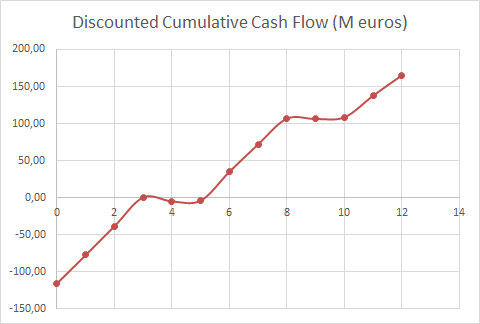
\includegraphics{DCCF.jpg}

In that graphic, it can be seen what has just been explained. In year 15 there will be a new decrease, but this time, its lowest point (locally) will be positive, and from that point, there will always be a positive balance. 

\subsection{Internal Rate of Return (IRR)}
The internal rate of retorn is the interest rate at which the Net Present Value of all the cashflows is equal to zero. This is used to evaluate the attractiveness of a project. If the Internal Rate of Return of a project exceeds a company's required rate of return, the project is desirable, and if on the other hand the IRR falls below the required rate of return, the project should be rejected.

For the study carried on, the discount rate has been a 6\% anual. Because of what has been said in the NPV, since the NPV is negative, the IRR will be a smaller quantity. According to the theory, the project should be rejected. But once again, because of the re-launching of the tenth year, it is not a good indicative figure. It should have been a better idea to perform a 9 or 11 years analysis, but it was also interesting to do a economical study of the first two completes lifes of the satellites. 

Changing manually the parameter d of the table, it is found that for a discount ratio of 3.84\%, the NPV is zero, which means that this is the IRR. It is smaller than the actual discount ratio, just as was predicted and explained. 








